\id{IRSTI 47.09.48}{}

{\bfseries IMPORTANCE OF MXENE NANOCOMPOSITES IN THE DETECTION}

{\bfseries OF HEAVY METALS}

{\bfseries D.B.
\begin{figure}[H]
	\centering
	
\includegraphics[width=0.8\textwidth]{media/chem2/image8}
	\caption*{}
\end{figure}

, Y.
\begin{figure}[H]
	\centering
	
\includegraphics[width=0.8\textwidth]{media/chem2/image9}
	\caption*{}
\end{figure}

Zh.S.
\begin{figure}[H]
	\centering
	
\includegraphics[width=0.8\textwidth]{media/chem2/image9}
	\caption*{}
\end{figure}

N.A.
\begin{figure}[H]
	\centering
	
\includegraphics[width=0.8\textwidth]{media/chem2/image9}
	\caption*{}
\end{figure}

{\bfseries ,}

{\bfseries D.A. Karazhanova}
\begin{figure}[H]
	\centering
	
\includegraphics[width=0.8\textwidth]{media/chem2/image10}
	\caption*{}
\end{figure}

Zh.R.
\begin{figure}[H]
	\centering
	
\includegraphics[width=0.8\textwidth]{media/chem2/image11}
	\caption*{}
\end{figure}


\emph{\textsuperscript{1}Abai Kazakh National Pedagogical University»,
Almaty city, Kazakhstan}

\textsuperscript{\envelope }Corresponding-author:
\emph{\href{mailto:konarbay98@bk.ru}{\nolinkurl{konarbay98@bk.ru}},
\href{mailto:Rysgul_01_88@mail.ru}{\nolinkurl{Rysgul\_01\_88@mail.ru}}}

One of the strongest and most common chemical pollution is its
environmental pollution with heavy metals. Heavy metals are actively
involved in biological processes, which are part of many enzymes. The
toxicity of heavy metal ions causes a number of harm to environmental
components and human health. That is why the detection of heavy metals
is so important. The creation of a reliable and effective system for
detecting heavy metals is crucial. And traditional detection methods are
often not enough to meet the current needs. Therefore, the use of
electrochemical sensors in the detection of heavy metals is currently
taking an important place. Electrochemical sensors have become a
promising area of research due to their unique capabilities. Improving
the detection efficiency of electrochemical sensors is the main area of
research. The leading strategy for significantly improving detection
performance involves adding nanomaterials to electrochemical sensors.
This review compares MXene nanocompasites with the achievements of
nanomaterials in the field of electrochemical sensors in recent years.
This makes it possible to obtain new ideas for the manufacture of
electrochemical sensors with high sensitivity and low detection
threshold. We believe that knowing and combining the benefits of
different nanomaterials to produce innovative electrode modification
materials can eliminate the risk of heavy metal ions in many food,
environmental and other industries.

{\bfseries Keywords:} heavy metals, electrochemical sensors, nanomaterials,
modification, MXene nanocomposites.

{\bfseries АУЫР МЕТАЛДАРДЫ АНЫҚТАУДА MXENE НАНОКОМПОЗИТТЕРДІҢ МАҢЫЗЫ}

{\bfseries Д.Б. Қонарбай\textsuperscript{\envelope } ,} {\bfseries Ы.
Бақыткәрім\textsuperscript{\envelope }}, {\bfseries Ж.С. Мұқатаева,} {\bfseries Н.А.
Шадин,}

{\bfseries Д.А. Каражанова, Ж.Р. Кожагулова}

\emph{\textsuperscript{1}Абай атындағы Қазақ ұлттық педагогикалық
университеті», Алматы, Қазақстан,}

e-mail:
\emph{\href{mailto:konarbay98@bk.ru}{\nolinkurl{konarbay98@bk.ru}},
\href{mailto:Rysgul_01_88@mail.ru}{\nolinkurl{Rysgul\_01\_88@mail.ru}}}

Ең күшті және ең көп таралған химиялық ластанудың бірі - ол қоршаған
ортаның ауыр металдармен ластануы. Ауыр металдар көптеген ферменттердің
құрамына кіретін биологиялық процестерге белсенді қатысады. Ауыр металл
иондарының уыттылығы қоршаған орта компоненттеріне және адам
денсаулығына бірқатар зиянын келтіреді. Сондықтан да ауыр металдарды
анықтау өте маңызды болып табылады. Ауыр металдарды анықтау үшін сенімді
және тиімді жүйені құру қажет. Ал дәстүрлі анықтау әдістері көбінесе
қазіргі қажеттіліктерді қанағаттандыру үшін жеткіліксіз. Сондықтанда
қазіргі кезде ауыр металдарды анықтауда электрохимиялық сенсорларды
қолдану маңызды орын алып отыр. Электрохимиялық сенсорлар өзінің ерекше
мүмкіндіктерінің арқасында зерттеудің перспективалық бағытына айналды.
Электрохимиялық сенсорларды анықтау тиімділігін арттыру зерттеудің
негізгі бағыты болып табылады. Анықтау өнімділігін айтарлықтай
жақсартудың жетекші стратегиясы наноматериалдарды электрохимиялық
сенсорларға қосуды қамтиды. Бұл шолу MXene нанокомпазиттерін
соңғы жылдардағы электрохимиялық сенсорлар саласындағы
наноматериалдардың жетістіктерін салыстырады. Бұл жоғары
сезімталдығы бар және анықтау шегі төмен электрохимиялық
сенсорларды дайындау үшін жаңа идеялар алуға мүмкіндік береді.
Электродтарды модификациялау үшін инновациялық материалдар алу
үшін әртүрлі наноматериалдардың артықшылықтарын білу және
біріктіру көптеген азық-түлік, экологиялық және де басқа
салалардағы ауыр металл иондарының қаупін жоя алады деген
ойдамыз.

{\bfseries Түйін сөздер:} Ауы{\bfseries }р металдар, электрохимиялық
сенсорлар, наноматериалдар, модификация, MXene нанокомпозиттері.

{\bfseries ВАЖНОСТЬ НАНОКОМПОЗИТОВ MXENE ДЛЯ ОПРЕДЕЛЕНИЯ ТЯЖЕЛЫХ
МЕТАЛЛОВ}

{\bfseries \textsuperscript{}Д.Б.}
{\bfseries Кон}{\bfseries арбай\textsuperscript{\envelope } , \textsuperscript{}Ы.
Бакыткарим\textsuperscript{\envelope } ,} \textsuperscript{}{\bfseries Ж.С.
Мукатаева, \textsuperscript{}Н.А.Шадин,}

{\bfseries \textsuperscript{}Д.А. Каражанова, \textsuperscript{}Ж.Р.
Кожагулова}

\emph{\textsuperscript{}Казахский национальный педагогический
университет имени Абая», г. Алматы, Казахстан,}

\emph{e-mail:
\href{mailto:konarbay98@bk.ru}{\nolinkurl{konarbay98@bk.ru}},
\href{mailto:Rysgul_01_88@mail.ru}{Rysgul\_01\_88@mail.ru}}

Одним из самых сильных и распространенных химических загрязнений
является загрязнение окружающей среды тяжелыми металлами. Тяжелые
металлы активно участвуют в биологических процессах, входя в
состав многих ферментов. Токсичность ионов тяжелых металлов
наносит ряд повреждений компонентам окружающей среды и здоровью
человека. Именно поэтому обнаружение тяжелых металлов так важно.
Необходимо создать надежную и эффективную систему для обнаружения
тяжелых металлов. А традиционных методов обнаружения зачастую
недостаточно для удовлетворения современных потребностей. Поэтому
использование электрохимических сенсоров для обнаружения тяжелых
металлов в настоящее время занимает важное место.
Электрохимические сенсоры стали перспективным направлением
исследований благодаря своим уникальным возможностям. Повышение
эффективности обнаружения электрохимических сенсоров является
основным направлением исследований. Ведущей стратегией для
значительного повышения эффективности обнаружения является
добавление наноматериалов в электрохимические сенсоры. В данном
обзоре сравниваются нанокомпозиты MXene с достижениями
наноматериалв в области электрохимических сенсоров за последние
годы. Это позволяет получить новые идеи для изготовления
электрохимических сенсоров с выской чувствительностью и низким
порогом обнаружения. Мы считаем, что знание и комбинирование
преимуществ различных наноматериалов для создания инновационных
материалов для модификации электродов может устранить опасность
ионов тяжелых металлов во многих пищевых, экологических и других
отраслях промышленности.

{\bfseries Ключевые слова:} тяжелые металлы, электрохимические
сенсоры, наноматериалы, модификация, нанокомпозиты MXene.

{\bfseries Introduction.} Heavy metals are particularly biodegradable
pollutants. They enter aquatic ecosystems, enter water and
sediment phases, accumulate in organisms, and even at low levels
cause a number of serious diseases and disorders {[}1-4{]}. For
example, neurological, cardiovascular, respiratory and
reproductive diseases {[}5{]}. Heavy metals in the environment
pose a serious threat to wildlife and human health because they
are bioavailable and can be absorbed and enriched in food
{[}6{]}. Toxic metals are largely distributed into the
environment. The distribution of heavy metals by wind in the
form of particles or vapor depends on their physical state. The
meta-components move from the atmosphere to the soil or water
surface, resulting in environmental pollution. Industrial
wastewater is a major source of metal pollution in the
hydrosphere. Wastewater containing toxic heavy metals like
nickel, lead, copper, chromium, cadmium, and arsenic poses
environmental and health hazards {[}7{]}. Heavy metals affecting
human health include elements such as mercury, nickel, lead,
chromium, cadmium, aluminum and copper {[}8{]}. Heavy metals in
water, air and soil can be transferred to plants, aquatic
organisms and organisms and then enter the food chain and
pose a threat to human health {[}9{]}.

Year after year, the population around the world is growing. As
the world' s population grows, the demand for
food, drinking water and many other industries increases. Due
to the increased demand, the quality requirements for food and
drinking water are increasing. To ensure consumer safety, we
must detect harmful substances present in very low
concentrations. One of the most commonly used methods today is
the use of electrochemical sensors.

Electrochemical sensors are tools for detecting and counting
heavy metals because they tend to be highly specific, sensitive,
inexpensive and portable. This makes them valuable for small
and mobile remote applications. Since complete elimination of
food and drinking water contamination may not seem possible in
the near future, assessment of legal limits should always be
considered in the context of general nutrition, especially in the
case of children. Ongoing research continues to improve sensor
performance, enhance detection capabilities, and address
calibration, interference, and sample preparation issues, further
advancing the development of electrochemical sensors in food
safety applications {[}10{]}.

The world of sensors is diverse and due to this, it is developing
at a rapid pace. Due to continuous technological improvement it is
becoming more and more in demand. Electrochemical sensors are a
convenient solution for variable analyzer detection due to their
low cost and availability and are widely used in agriculture,
food and oil industry as well as in environmental and biomedical
fields. Electrochemical sensors have long been required for the
study of biological substances. The sensors are characterized
not only by their durability, high sensitivity and accuracy,
but also by their low cost, speed and simplicity. Many
nanomaterials have been obtained in more than two decades.
Specific metals, conducting polymers, metal oxides and
organometallic and carbon-based nanomaterial structures.
Nanomaterials contribute to the analytical performance included in
electrochemical analysis. This modification increases the payload
capacity by utilizing recognition molecules such as enzymes,
antibodies and aptamers as well as bioinspired receptors that
can accurately and efficiently capture the target, thereby
increasing the specificity of electrochemical sensors {[}11{]}.

Electrochemistry-an important quantitative analysis strategy for
testing various biochemical entities such as proteins,
metabolites, neurotransmitters, electrolytes, heavy metals, etc.
Further, demonstrating wide applications in the fields of private
health care, public health, clinical diagnostics, food safety
and environmental analysis {[}12-14{]}. Generally, a complete
electrochemical conversion system usually consists of two parts:
sensing electrodes and electrochemically sensitive circuits. The
former is used to convert biochemical signals into electrical
signals. The latter uses various electrochemical test methods to
excite the electrodes with voltage, collect, process, analyze
the data and transmit them as electrical signals {[}15,16{]}.

MXenes'{} electrical conductivity, rich surface
chemistry and high aspect ratio are attractive characteristics
for sensor processing . The ideal sensor has high performance,
low detection , low production cost, low hysteresis, fast and
efficient processing reaction, as well as fast recovery
properties during reuse . Pressure and deformation sensors are
production responsible in a wide pressure range and require high
performance in thousands of deformation cycles. The cycles
require high resistance in thousands of deformation cycles. The
sensors demonstrated this product when made from MXenes,
mxen/polymer nanocomposites, and mixed two-dimensional (2D)
mxen-based heterostructures. Examples: silver nanoparticles,
carbon nanotubes, and graphene oxide nanoparticles are 0D, 1D,
and 2D nanoparticles that were combined with MXene and used to
create Mxene-based 2D heterostructures {[}17{]}.The latter
includes mxen and heterostructure of 0D, 1D or 2D nanomaterials.
These are heterostructures, as well as the detection of pure
MXene and MXene /polymer nanocomposites and toxic compounds in
food, monitoring of human movements and health status, gas and
condition measurement, voice recognition and other input in
sensory systems. appropriateness, voice recognition and other
aspects {[}18{]}.

{\bfseries Table 1- Lists many MXene-based sensors and their
corresponding applications {[}19{]}}

% \begin{longtable}[]{@{}
%   >{\raggedright\arraybackslash}p{(\columnwidth - 2\tabcolsep) * \real{0.5001}}
%   >{\raggedright\arraybackslash}p{(\columnwidth - 2\tabcolsep) * \real{0.4999}}@{}}
% \toprule\noalign{}
% \begin{minipage}[b]{\linewidth}\raggedright
% {\bfseries Nanocomposite components}
% \end{minipage} & \begin{minipage}[b]{\linewidth}\raggedright
% {\bfseries Application}
% \end{minipage} \\
% \midrule\noalign{}
% \endhead
% \bottomrule\noalign{}
% \endlastfoot
% {\bfseries Ti\textsubscript{3}C\textsubscript{2} / reduced graphene
% oxide} & Pressure sensor \\
% {\bfseries Ti\textsubscript{3}C\textsubscript{2}/ Ag nanowire} & Strain
% sensor \\
% {\bfseries Ti\textsubscript{3}C\textsubscript{2} / chitosan} & Biosensor
% for detecting pesticides \\
% {\bfseries Ti\textsubscript{3}C\textsubscript{2} / Nafion} & Detecting
% nitrile ions \\
% {\bfseries Ti\textsubscript{3}C\textsubscript{2} / PANI} & Ethanol,
% methanol, ammonia, and acetone detection \\
% {\bfseries Ti\textsubscript{3}C\textsubscript{2} / polyurethane} &
% Stretchable strain sensing fabric \\
% {\bfseries Ti\textsubscript{3}C\textsubscript{2}/ poly(vinylidene
% fluoride-trifluoroethylene)} & Capacitive pressure sensor \\
% {\bfseries Ti\textsubscript{3}C\textsubscript{2} / natural
% microcapsules} & Epidermal flexible pressure sensors \\
% {\bfseries Ti\textsubscript{3}C\textsubscript{2} /
% poly(dimethylsiloxane)} & Skin conformal sensors for health
% monitoring \\
% {\bfseries Ti\textsubscript{3}C\textsubscript{2} / gold nanoparticles}
% & Glucose detection biosensor \\
% {\bfseries Ti\textsubscript{3}C\textsubscript{2} and
% TiO\textsubscript{2}} & H\textsubscript{2}O\textsubscript{2}
% detection \\
% {\bfseries hollow MXene spheres/ reduced graphene} & Piezoresistive
% pressure sensor \\
% {\bfseries Ti\textsubscript{3}C\textsubscript{2} / ink} & Strain sensor
% for health monitoring \\
% \end{longtable}

MXene performance in sensor systems depends on the type and
concentration of surface functional groups (hydroxyl, oxygen,
fluorine, chlorine). For example, the simulation results showed
that oxygen-ending MXene has excellent performance for ammonia
detection, while hydroxyl-ending MXene has better performance
for ethanol detection.To further improve the electrochemical
performance of electrochemical sensors, sensitive Nanomaterials
and 2D materials have been introduced due to high
electrocatalytic effect and high electrical conductivity
{[}20{]}.

Mxene is a novel 2D material with a rare combination of
properties such as electrical and metallic conductivity,
hydrophilicity, biocompatibility and large surface area ,
convenient size customization, rich surface chemistry,
flexibility, and layered structure. Due to its versatile
properties, MXene is considered as a building material for future
materials and devices {[}21{]}.

As an electrode material, MXene is a potential candidate for
synthesis for various energy storage devices such as
supercapacitors and batteries. Composites based on metal oxides
and metal sulfides are the most effective electrode materials
for supercapacitor electrodes. Research was carried out to
improve the properties of MXene-based composites {[}22 {]}.

\begin{figure}[H]
	\centering
	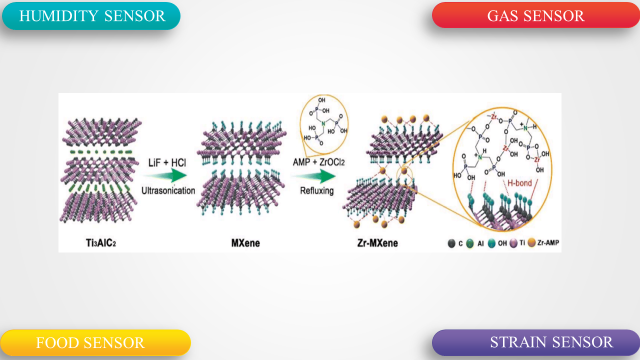
\includegraphics[width=0.8\textwidth]{media/chem2/image12}
	\caption*{}
\end{figure}


{\bfseries Figure 1 - Types of Mxene-based sensors {[}19{]}}

{\bfseries Table 2 - Advantages and disadvantages of MXepe materials}

% \begin{longtable}[]{@{}
%   >{\raggedright\arraybackslash}p{(\columnwidth - 4\tabcolsep) * \real{0.1339}}
%   >{\raggedright\arraybackslash}p{(\columnwidth - 4\tabcolsep) * \real{0.4030}}
%   >{\raggedright\arraybackslash}p{(\columnwidth - 4\tabcolsep) * \real{0.4631}}@{}}
% \toprule\noalign{}
% \begin{minipage}[b]{\linewidth}\raggedright
% \end{minipage} & \begin{minipage}[b]{\linewidth}\raggedright
% {\bfseries Advantages}
% \end{minipage} & \begin{minipage}[b]{\linewidth}\raggedright
% {\bfseries Disadvantages}
% \end{minipage} \\
% \midrule\noalign{}
% \endhead
% \bottomrule\noalign{}
% \endlastfoot
% {\bfseries MXene} & -Stability
% 
% - Optical properties
% 
% - Good hydrophilicity
% 
% - Conductivity
% 
% -Outstanding mechanical properties
% 
% - Thermal effect
% 
% - Excellent biocompatibility
% 
% - High electrical conductivity & -The preparation process of MXene
% sensitive materials must be further developed
% 
% - The abundant functional groups on the surface of MXene
% materials endow them with customizable optical and electrical
% properties, but also bring new challenge \\
% \end{longtable}

{\bfseries Materials and methods.} \emph{Nanocomposite
WO\textsubscript{3}/Mxene}

Al-Zoha Wapsi and others {[}23{]} used a hydrothermal method
for the synthesis of tungsten oxide nanorods. The synthesis of
WO\textsubscript{3}/MXene by a simple ultrasound method was
carried out. The samples obtained were characterized by
structural, spectral, morphological and elemental analysis. The
photocatalytic and antibacterial activity of synthesized samples,
these aspects are discussed in detail. Max
(Ti\textsubscript{3}AlC\textsubscript{2}) powder was used in a 50
ml Teflon container to synthesize MXene with the formula
Ti\textsubscript{3}C\textsubscript{2}Tx used. To synthesize MXene
with the formula Ti\textsubscript{3}C\textsubscript{2}Tx in a 50 ml
Teflon container. For MXene synthesis, 10 ml of HF is poured
into a Teflon container and then released into a suction cup .
Then, instead of low HF, MAX 0.5 g powder and a pinch were
added. The mixture was equipped with magnetic instruments for
an hour at room temperature.

The combustion optimization of the mixture was carried out at
the installation temperature for 24 hours with magnetic power.
Deionized (DI) water was added to dilute the product, and MXene
was obtained by centrifugation at more than 5000 rpm. The
washing of these deposits was performed until the PH reached 6.
The Aqueous Dispersion was carried out using a PTFE membrane by
vaum filtration. Filtrate is here.

For FESEM analysis, samples were sprayed with gold for 120
seconds at a current of 15 ma. Figure-2 A, B WO\textsubscript{3}
and WO\textsubscript{3}/MXene nanocomposite morphology control.
Figure-2 - (a) illustrates the block/stick pattern morphology of
WO\textsubscript{3}. Figure-2 (b) MXene WO\textsubscript{3} is
defined as impregnated with nano wires. MXene Nano sample
structure formation in Figure 2 - (c). The size of the
WO\textsubscript{3} was about 13 nm, after the reduction of
FESEM. The MXene layer was estimated at \textasciitilde175 nm on
an additional micro-image. For FESEM analysis, the samples were
subjected to gold spraying for 120 seconds at a current of 15
ma. Figure-2 A,B WO\textsubscript{3} and WO\textsubscript{3}/MXene
nanocomposite morphology control. Figure 1 shows the morphology
of WO\textsubscript{3} with a block or stick inscription. Figure -
2 (b) MXene WO\textsubscript{3} is detected in an impregnated
manner with nano wires. Figure 2 (c) shows the MXene formation
of the nanoscale structure. The size of the WO\textsubscript{3}
volume was about 13 nm, which is after the reduction of FESEM.
In the micrograph, the size of the mxen layer was 175 nm.

\begin{figure}[H]
	\centering
	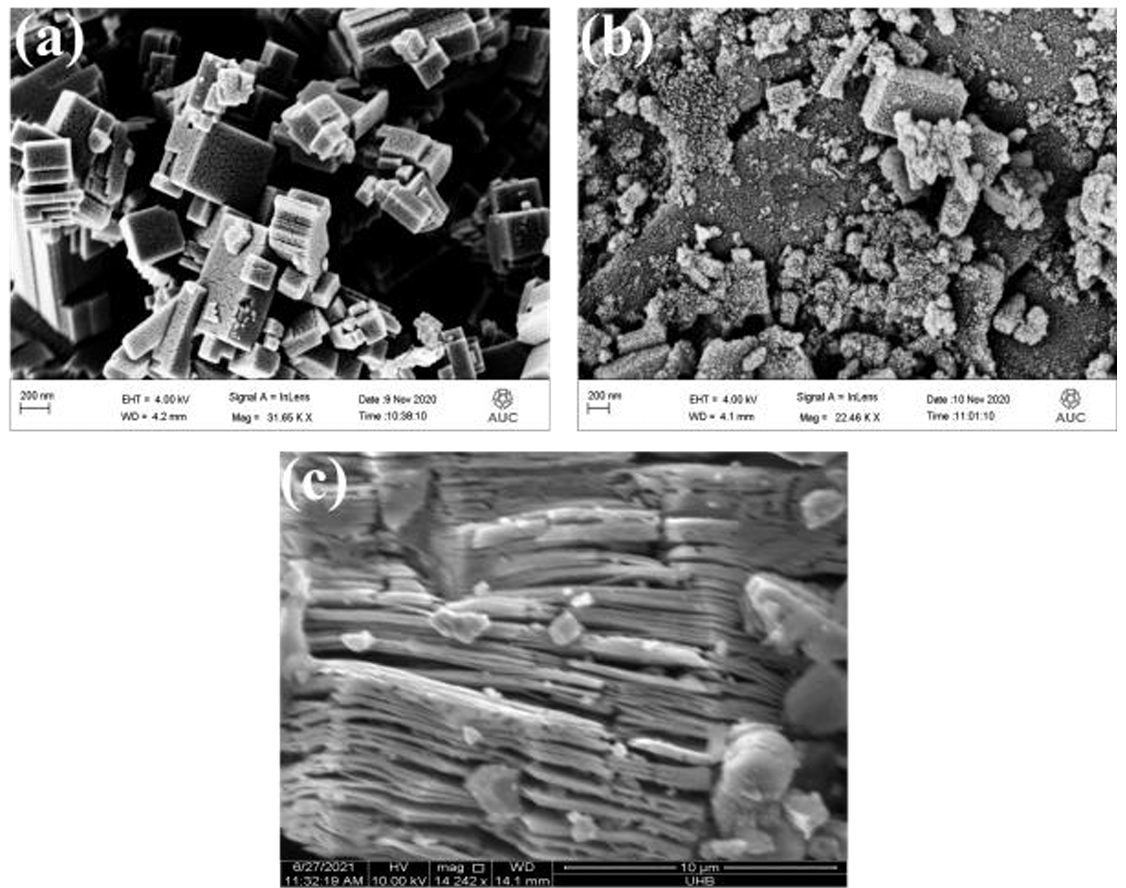
\includegraphics[width=0.8\textwidth]{media/chem2/image13}
	\caption*{}
\end{figure}


{\bfseries Figure 2 - FESEM images (A) WO\textsubscript{3}, (b)
WO\textsubscript{3}/MXene nanocomposite and (c) MXene {[}23{]}}

In this paper, A.Z. Warsi, Aziz, F. Zulfiqar et al. prepared
WO\textsubscript{3}, MXene and WO\textsubscript{3}/MXene
nanocomposite which showed potential applications in biological
and environmental remediation. WO\textsubscript{3}, MXene and
WO/Mxene nanocomposite were synthesized by hydrothermal method,
wet chemical etching and sonication, respectively. XRD, XRD,
FTIR, EDX and FESEM were used to determine the structural,
spectral, elemental and morphological characteristics of the
synthesized samples, respectively. BET analysis was performed to
determine the surface area. The photocatalytic degradation of
methylene blue using WO\textsubscript{3}, MXene and
WO\textsubscript{3}/MXene nanocomposites was 99\%, 54\% and 89\%,
respectively. The photocatalytic activity of WO\textsubscript{3}
was significant. MXene is a two-dimensional material with very
low photocatalytic activity, which acts only as an auxiliary
material to enhance the photocatalytic ability of the composite
with WO\textsubscript{3}.

The prepared samples also showed good antibacterial activity
against bacteria of positive strain; in case of negative strains,
WO\textsubscript{3}, MXene and WO\textsubscript{3}/MXene
nanocomposite showed antibacterial activity at high concentrations
{[}23{]}.

\emph{Bi\textsubscript{2}S\textsubscript{3}/MXene nanocomposite}

In a study {[}24{]} by S. Sinha, A. Raucci et al. developed a
novel electrochemical sensing platform using
Bi\textsubscript{2}S\textsubscript{3}/MXene nanocomposite. The
modified shape, composition and electrical characteristics of the
prepared composites and their electrodes were studied by various
electrochemical methods SEM, XRD, XPS and others. A 1 mg/ml
solution of Bi\textsubscript{2}S\textsubscript{3}/Mxene
nanocomposite was prepared by dispersing DI (deionized) in water.
This standard solution was the base of the electrode
modification process. This initial solution base served as the
electrode modification process. An 8 μL dispersion of
Bi\textsubscript{2}S\textsubscript{3}/Mxene nanocomposites was
carefully placed on the surface of SPE to modify the electrode.
Bi\textsubscript{2}S\textsubscript{3}/Mxene nanocomposites were
synthesized directly by microwave-assisted hydrothermal method.
The figure below shows the accumulation of 3 - (A) {[}24{]}
Bi\textsubscript{2}S\textsubscript{3} nanoparticles. These are
granular nanoparticles with diameters ranging from 70 to 100 nm.
And figure 3 - (B) shows the MXene SPE image. This figure
shows the complex layered lamellar structure of MXene after
removing the Al layers from the MAX phase. SEM image of
Bi\textsubscript{2}S\textsubscript{3}-MXene nanocomposites are
shown in Fig.3C and 3D (small and large scale).

\begin{figure}[H]
	\centering
	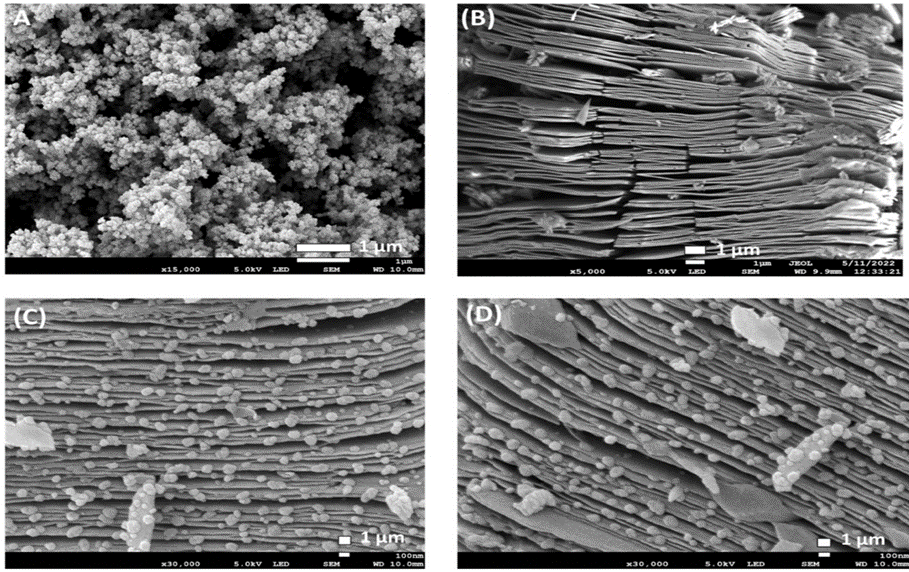
\includegraphics[width=0.8\textwidth]{media/chem2/image14}
	\caption*{}
\end{figure}


{\bfseries Figure 3 - Structural characteristics of (A)
Bi\textsubscript{2}S\textsubscript{3}; (B) MXene; (C)
Bi\textsubscript{2}S\textsubscript{3}-MXene nanocomposite at low
magnification; (D) Bi\textsubscript{2}S\textsubscript{3}-MXene
nanocomposite at high magnification {[}24{]}}

The uniform growth of Bi\textsubscript{2}S\textsubscript{3}
nanoparticles in MXene layers growth of
Bi\textsubscript{2}S\textsubscript{3} nanoparticles (F and OH) was
due to the presence of electronegative functional groups. The
synergistic effect of Bi\textsubscript{2}S\textsubscript{3}
nanoparticles and MXene can improve the electrochemical
performance. First, MXene provides a highly conductive platform
for the uniform growth of Bi\textsubscript{2}S\textsubscript{3}
nanoparticles. This leads to reduced agglomeration of
Bi\textsubscript{2}S\textsubscript{3} nanoparticles and increased
number of detection sites for the target analyte {[}25{]}.
Secondly, MXene is highly conductive, which leads to an increase
in charge between Bi\textsubscript{2}S\textsubscript{3}
nanoparticles and the electrolyte {[}26{]}. In addition, the
oxidation resistance property demonstrated by MXene plays an
important role in protecting Bi\textsubscript{2}S\textsubscript{3}
nanoparticles from corrosion {[}27{]}. The binding of MXene and
Bi\textsubscript{2}S\textsubscript{3} nanoparticles can lead to
improved performance in Zn(II) detection.

\emph{The study focuses on the synthesis of a composite made of
MoO\textsubscript{2}@Mo\textsubscript{2}C-MXene.}

This article discusses the new CdS/MoO\textsubscript{2}
photocatalyst @Mo\textsubscript{2}C-MXene developed by You Jin,
Huizhuan Jing, Libo Wang, Qianku Hu and Aigo Zhou. 0.2 g of
NaBF4 (99.9\%, McLean, China) was used as a guiding reagent,
dissolved in 15 ml of 1.0 m HCl solution (36-38\% C/a , Yantai
Shuangshuang Chemical, China) and stirred for 30 minutes. The
temperature of the hydraulic system is maintained at 180 ℃ for
24 hours every day. The temperature of the hydraulic system is
kept at 180 ℃ for 24 hours every day. Subsequently,
MoO\textsubscript{2}@Mo\textsubscript{2}C-MXene Composite powders
were collected, subjected to washing with deionized water and
ethanol to achieve a neutral reaction, and then dried for 12
hours at 60 ℃ for 12 hours under vacuum conditions.

CdS / MoO\textsubscript{2}@ Mo\textsubscript{2}C photocatalysts
were effectively synthesized by a two-stage hydrothermal method .
In this system, a sediment formed on the surface of the CdS
MoO\textsubscript{2}@Mo\textsubscript{2}C-MXene Composite, forming
an acanthospheric structure. CdS /
MoO\textsubscript{2}@Mo\textsubscript{2}C(CMM5) showed an
exceptional H\textsubscript{2} generation rate of 22,672
µmol/(g-h) in visible light under optimal conditions, which is
11.8 times higher than CdS. full row,
Moo\textsubscript{2}@Mo\textsubscript{2}C-MXene binary co-catalyst
using CdS using high photocatalytic activity of productive
H\textsubscript{2} generation with Mo\textsubscript{2}C MXene as
the only co-catalyst. Experimental effects the
CdS/Mo\textsubscript{2}C system effects work with CdS
/Mo\textsubscript{2}C with high photophysical and
photoelectrochemical properties to serve as an electronic bridge
between CdS and Mo\textsubscript{2}C MXene with improved
electrical conductivity . "no," he said. In addition to the
CdS/Mo\textsubscript{2}C script, the CdS conduction band (CB) is
a place to charge when MoO\textsubscript{2}@Mo\textsubscript{2}C
is MXene bound. This effectively limits the re - diffusion of
Altered electrons into CdS , thus facilitating the operation of
recombination. The band forbidden to control over
CdS/MoO\textsubscript{2}@ Mo\textsubscript{2}C makes it easy to
absorb visible light. This CdS/Mo\textsubscript{2}C {[}28{]}
element restored a new photocatalytic system with the formation
of a binary H\textsubscript{2} co-catalyst.

The process of preparing Ti3C2 involves the use of various
chemical and physical methods to create a highly durable and
efficient material: The crude powder (50 g) was weighed in the
following ratio TiC:Ti:Al = 3.6:1.4:1 and then placed in a
Teflon ball mill. Anhydrous ethanol was then added to the ball
mill tank as a ball grinding aid and zirconium dioxide (5 nm
diameter) as a grinding medium. The mass ratio of raw material
powder, anhydrous ethanol and pellets should be 1:1:3. The
ball was placed in a grinding vessel and the powder mixture
was pulverized at 300 rpm for 4 hours. Next, a ball mill was
used to obtain a homogeneous mixture and then it was transferred
into a petri dish. The mixture was dried in an oven at 40°C for
24 hours, then sintered in a corundum crucible without pressure.

After the reaction was completely completed, the sintering
furnace was allowed to cool down naturally to room temperature
and a Ti\textsubscript{3}AlC\textsubscript{2}
cer\textsubscript{}amic block was obtained by pressureless
sintering. A high-energy ball mill was used to completely
pulverize the Ti\textsubscript{3}AlC\textsubscript{2} ceramic
block obtained by pressureless sintering i+n the previous step;
finally, the desired Ti\textsubscript{3}AlC\textsubscript{2}
powder was successfully obtained. At room temperature, 5 g of
Ti\textsubscript{3}AlC\textsubscript{2} powder was slowly added to
80 mL of 40 wt\% HF and left to react for 24 h under magnetic
stirring at 1200 rpm. The above corrosion products were
purified with deionized water until the pH of the supernatant
became \textgreater{} 6 after centrifugation. The substrate was
lyophilized to obtain Ti\textsubscript{3}C\textsubscript{2} powder.

Preparation of the PANI-Ti\textsubscript{3}C\textsubscript{2}
composite: first, 0.2 g of Ti\textsubscript{3}C\textsubscript{2}
powder was dispersed in 30 mL of 1M hydrochloric acid solution,
then ultrasonic dispersion was carried out for 1 h until a
homogeneous suspension was obtained. Second, 100 μL of pure
aniline (ANI) obtained by distillation was added to the
suspension and dispersed by ultrasonic dispersion for 1h. Then,
0.335 g of ammonium persulfate (APS) was dissolved in 30 mL of 1
M hydrochloric acid solution and added dropwise to the above
solution. Finally, the solution was placed in an ice bath and
stirred at 0°C for 6 hours. After reaction, the reaction product
was washed with ultrapure water 5 times. After purification,
the reaction product was lyophilized to obtain
PANI-Ti\textsubscript{3}C\textsubscript{2} nanocomposite {[}29{]}.

Figure 1A shows the X-ray diffraction patterns of the obtained
PANI, Ti\textsubscript{3}C\textsubscript{2} and
PANI-Ti\textsubscript{3}C\textsubscript{2}. The figure shows that
the X-ray diffraction peak of PANI at 2 theta=20.5° corresponds
to the surface (020) of the PANI crystal. The diffraction peak
of Ti\textsubscript{3}C\textsubscript{2} on the crystal plane
(002) is shifted to the left along the x-axis from that of the
original phase Ti\textsubscript{3}AlC\textsubscript{2}, which
makes the characteristic peak of
Ti\textsubscript{3}C\textsubscript{2} weaker and wider.

This X-ray diffraction pattern can show that the degree of
crystallinity and the degree of structural order of
Ti\textsubscript{3}C\textsubscript{2} are greatly reduced. In the
X-ray radiograph of Ti\textsubscript{3}C\textsubscript{2}, the
diffraction peaks at 2 theta =7.1°, 17°, 28°, 35°, 41° and
61° correspond to the crystal planes (002), (006), (008), (
0010), (0012) and (110), respectively. Compared with the
Ti\textsubscript{3}C\textsubscript{2} XRD, the
PANI-Ti\textsubscript{3}C\textsubscript{2} XRD shows a new
diffraction peak at 2 theta =20.7° corresponding to (020)
crystal surface of PANI. The XRD peak of
PANI-Ti\textsubscript{3}C\textsubscript{2} at 2 theta =26°
corresponds to TiO\textsubscript{2}. This value is due to the
fact that a small amount of Ti\textsubscript{3}C\textsubscript{2}
is oxidized by the addition of ammonium persulfate, an oxidizing
agent, during the preparation of the
PANI-Ti\textsubscript{3}C\textsubscript{2} composite material.
Thus, the phase analysis shows the successful preparation of
PANI-Ti\textsubscript{3}C\textsubscript{2} nanocomposite.
Ti\textsubscript{3}C\textsubscript{2} can easily immobilize
enzymes/proteins on its surface, thus acting as a promising
support to achieve DET with accelerated electrode kinetics, low
detection limits, and high sensitivity and selectivity {[}30{]}.

\begin{figure}[H]
	\centering
	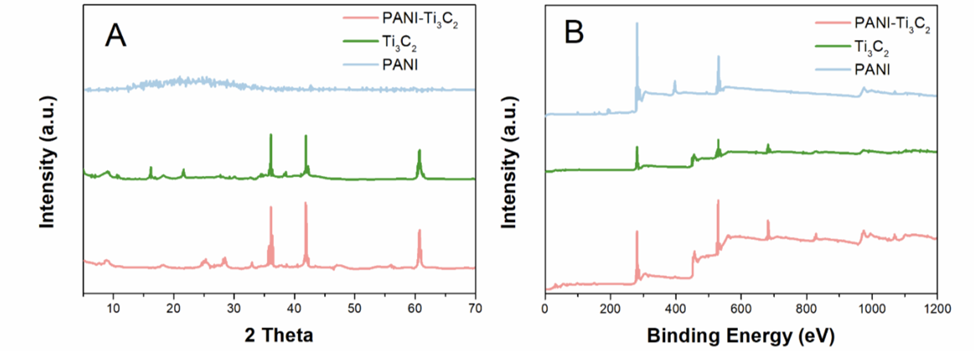
\includegraphics[width=0.8\textwidth]{media/chem2/image15}
	\caption*{}
\end{figure}


{\bfseries Figure 4 - (A) XRD patterns of PANI,
Ti\textsubscript{3}C\textsubscript{2} and
PANI-Ti\textsubscript{3}C\textsubscript{2}. (B) XPS spectras of
PANI, Ti\textsubscript{3}C\textsubscript{2} and
PANI-Ti\textsubscript{3}C\textsubscript{2} {[}30{]}}

Figure 1B shows the XRD spectra of the obtained PANI,
Ti\textsubscript{3}C\textsubscript{2} and
PANI-Ti\textsubscript{3}C\textsubscript{2}. As can be seen from
the figure, characteristic peaks C1s, O1s, F1s and
Ti\textsubscript{2}p appear, proving the existence of
Ti\textsubscript{3}C\textsubscript{2}. At the same time, the
appearance of characteristic peaks O1s and F1s proves the
existence of functional groups -O, -OH and -F on the laminates of
Ti\textsubscript{3}C\textsubscript{2}. The appearance of C1s and
N1s peaks indicates the successful obtaining of PANI. Compared
with Ti\textsubscript{3}C\textsubscript{2} , the broad XPS
spectrum of PANI-Ti\textsubscript{3}C\textsubscript{2} shows N1s
peak, which further proves the successful preparation of
PANI-Ti\textsubscript{3}C\textsubscript{2} nanocomposites under
low temperature stirring conditions. The above results are in
agreement with the results of X-ray diffraction analysis. By the
integral approximation method, N1s -analysis of the RFES spectra
of the PANI-Ti\textsubscript{3}C\textsubscript{2}
nan\textsubscript{}ocomposite showed four characteristic peaks at
397.1 eV, 398.2 eV, 400.1 eV and 400.5 eV corresponding to the
imine structure (=NH-), amino group (-NH-). -), N atom (N-+) with
positron and protonated amino group, respectively. The results
show that the PANI-Ti\textsubscript{3}C\textsubscript{2}
nanocomposite was successfully obtained by low-temperature
oxidation reaction between Ti\textsubscript{3}C\textsubscript{2}
and aniline.

\emph{Ti\textsubscript{3}C\textsubscript{2}/TiO\textsubscript{2}/CuO
nanocomposites}

In experiments, researchers Li, Wang, and Sun dissolved copper
nitrate in deionized water and added
Ti\textsubscript{3}C\textsubscript{2} powder. The mixture was
incubated for 24 hours, dried, and then synthesized into
Ti\textsubscript{3}C\textsubscript{2}/TiO\textsubscript{2}/CuO
nanocomposites by annealing in an argon atmosphere at 500C for 30
minutes at a heating rate of 100C/min {[}31{]}. \hl{}

The fabrication of
Ti\textsubscript{3}C\textsubscript{2}/TiO\textsubscript{2}/CuO
ternary nanocomposites, consisting of
Ti\textsubscript{3}C\textsubscript{2} nanosheets,
TiO\textsubscript{2}, and CuO nanoparticles, was enhanced by
higher electron and hole separation efficiency compared to
TiO\textsubscript{2}, thereby improving their photocatalytic
activity {[}32{]}.

{\bfseries Discussion and results.} In this research, a series of
MXene-based nanocomposites including WO\textsubscript{3}/MXene,
Bi\textsubscript{2}S\textsubscript{3}/MXene, and
Ti\textsubscript{3}C\textsubscript{2}/TiO\textsubscript{2}/CuO were
synthesized and characterized. The obtained materials showed
high efficiency in various applications including photocatalytic
decomposition of organic pollutants and electrochemical detection
of heavy metals.

WO\textsubscript{3}/MXene:

\begin{itemize}
\item
  The morphology of the nanocomposite determined by FESEM revealed
  the presence of nanowires and layered structure.
\item
  The photocatalytic activity for methylene blue degradation
  reach-ed 89\%, which is higher than that of pure
  WO\textsubscript{3} (99\%) and significantly superior to that of
  MXene (54\%).
\item
  The nanocomposite demonstrated antibacterial activity against
  both positive and negative bacterial strains at high
  concentrations.
\end{itemize}

Bi\textsubscript{2}S\textsubscript{3}/MXene:

\begin{itemize}
\item
  The synergistic effect of Bi\textsubscript{2}S\textsubscript{3}
  and MXene was found to improve electrochemical performance,
  increase the number of active sites for analytical detection,
  and improve corrosion resistance.
\item
  The nanocomposite was successfully used for Zn(II) detection
  with high sensitivity.
\end{itemize}

Ti\textsubscript{3}C\textsubscript{2}/TiO\textsubscript{2}/CuO:

\begin{itemize}
\item
  The ternary nanocomposite showed enhanced photocatalytic
  activity due to the improved electron-hole separation ability.
\item
  The enhanced photocatalytic efficiency was attributed to the
  presence of TiO\textsubscript{2} and CuO, which enhanced the
  interaction with Ti\textsubscript{3}C\textsubscript{2}.
\end{itemize}

These results confirm the potential of MXene-based nanomaterials
in applications related to ecological remediation, biosensing and
environmental monitoring.

The results confirm the significant contribution of MXene-based
nanocomposites in improving the properties of sensors and
catalysts.

\emph{Photocatalytic activity:}

The high efficiency of WO\textsubscript{3}/MXene in the
photocatalytic decomposition of methylene blue can be explained by
the combination of MXene (high conductivity) and
WO\textsubscript{3} (active catalytic ability) properties. This
supports the hypothesis of a synergistic effect in the creation
of hybrid nanomaterials. Similarly,
Ti\textsubscript{3}C\textsubscript{2}/TiO\textsubscript{2}/CuO
nanocomposite demonstrates that the addition of CuO enhances the
charge separation ability, which is critical for photocatalysis.

\emph{Electrochemical detection:}

Bi\textsubscript{2}S\textsubscript{3}/MXene showed high sensitivity
to Zn(II), which is attributed to the increase of active centers
on the surface of MXene and its interaction with
Bi\textsubscript{2}S\textsubscript{3}. This result is in line with
current research in electrochemistry, where MXene is used as a
basic structure to improve the sensor response.

\emph{Lim}\emph{itations and prospects:}

Despite significant advances, difficulties in scaling up the
production of MXene nanocomposites should be considered.
Additional research is required to optimize synthesis methods and
material stability. Prospects for the use of these materials
include expanding their applications in environmental monitoring,
biomedicine, and water quality control.

Thus, the results of this study confirm the relevance and
promise of MXene-based nanocomposites for the development of
high-performance sensors and catalysts. Future research should
focus on improving the stability and fabrication processes of
these materials.

{\bfseries Conclusion.} This literature review is devoted to the
detection of heavy metals. Heavy metals are found in many
substances. There are many methods for detecting heavy metals.
Despite the large number of methods, we must use the most
effective of them. The article is written about the detection of
heavy metals using a sensor. In order to improve the sensor,
various nanomaterials are used. As a material, Mxene-based
nanocompasites were considered. Focused on MXene-based
nanocomposites and sensor research methods developed on their
basis. MXene materials are a stable single-phase structure
consisting of five or more atoms, and its elemental ratio can
be adjusted. MXene contains more transition metals, which
greatly optimizes material properties such as conductivity,
hardness, chemical stability, and bulk capacity.

{\bfseries References}

1. Singovszka E., Balintova M., Junakova N. The Impact of Heavy
Metals in Water from Abandoned Mine on Human Health//SN Applied
Sciences.-2020.-Vol.2:934

 DOI 10.1007/s42452-020-2731-2

2. Munir N., Jahangeer M., Bouyahya A., El Omari N., Ghchime R.,
Balahbib A., Aboulaghras S., Mahmood Z., Akram M., Ali Shah S.M.
Heavy Metal Contamination of Natural Foods Is a Serious Health
Issue: A Review//Sustainability.-2022.-Vol.14(1),161.
\href{https://doi.org/10.3390/su14010161}{DOI 10.3390/su14010161}

3. Ali H., Khan E. Trophic Transfer, Bioaccumulation, and
Biomagnification of Non-Essential Hazardous Heavy Metals and
Metalloids in Food Chains/Webs-Concepts and Implications for
Wildlife and Human Health//Human and Ecological Risk
Assessment.-2018.-Vol. 25(6).-P.1353-1376
\href{https://doi.org/10.1080/10807039.2018.1469398}{DOI
10.1080/10807039.2018.1469398}

4. Kumari P., Chowdhury A., Maiti S.K. Assessment of Heavy Metal
in the Water, Sediment, and Two Edible Fish Species of
Jamshedpur Urban Agglomeration, India with Special Emphasis on
Human Health//Human and Ecological Risk
Assessment.-2018.-Vol.24(7).-P.1-24

\href{https://doi.org/10.1080/10807039.2017.1415131}{DOI
10.1080/10807039.2017.1415131}

5. Sharma S., Nagpal A.K., Kaur I. Appraisal of Heavy Metal
Contents in Groundwater and Associated Health Hazards Posed to
Human Population of Ropar Wetland, Punjab, India and its
Environs//Chemosphere.-2019.-Vol. 227.- P.179 - 190.
\href{https://doi.org/10.1016/j.chemosphere.2019.04.009}{DOI
10.1016/j.chemosphere.2019.04.009}

6. Cheng S. Heavy metal pollution in China: Origin, pattern and
control// Enviro nmental Science

and Pollution Research.-2003.-Vol.10.-P.192-198.
\href{https://doi.org/10.1065/espr2002.11.141.1}{DOI
10.1065/espr2002.11.141.1}

7. Zykova I., Maksimuk N., Rebezov M., Kuznetsova E., Derkho M.,
Sereda T., Kazhibayeva G., Somova Y., Zaitseva T. Interaction
between Heavy Metals and Microorganisms during Wastewater
Treatment by Activated Sludge//ARPN Journal of Engineering and
Applied Sciences.-2020.-Vol.14(11).- P.2139--2145(2019).

8. Maria J.da Silva M, Paim A.P., I., Pimentel M.F., Cervera M.L.,
de la Guardia M. Determination of TOtal Mercury in Spanish Samples
of Baby Food, Fast Food, and Daily Meal//Journal of the
Brazilian Chemical Society.-2023.-Vol.34(4).-P.517-526.
\href{http://dx.doi.org/10.21577/0103-5053.20220125}{DOI
10.21577/0103-5053.20220125}

9. Qin G., Niu Z., Yu J., Li Z., Ma J., Xiang P. Soil heavy
metal pollution and food safety in China: Effects, sources and
removing technology//Chemosphere.-2021.-Vol.267:129205

\href{https://doi.org/10.1016/j.chemosphere.2020.129205}{DOI
10.1016/j.chemosphere.2020.129205}

10. Liliana A.N., Gheorghe G., Elena T., Sonia A. Electrochemical
sensors and biosensors: effective tools for detecting heavy
metals in water and food with possible implications for
children's health//International Journal of Electrochemical
Science, 19(2024).
\href{https://doi.org/10.1016/j.ijoes.2024.100643}{DOI
10.1016/j.ijoes.2024.100643}

11. Baranwal J., Barse B., Gatto G., Broncova G., Kumar A.
Electrochemical Sensors and Their Applications: A
Review//Chemosensors.-2022.-Vol.10(9):363.

\href{https://doi.org/10.3390/chemosensors10090363}{DOI
10.3390/chemosensors10090363}

12. Sammer-ul H., Zhang X. Microfluidics as an emerging platform
for tackling antimicrobial resistance (AMR): a review// Current
Analytical Chemistry.-2020.-Vol.16 (1).-P. 41-51

DOI 10.2174/1573411015666181224145845

13. Pohanka M. Screen printed electrodes in biosensors and
bioassays. A review// International Journal of Electrochemical
Science.-2020.-Vol.15 (11).-P.11024-11035.

DOI 10.20964/2020.11.19

14. Ozcelikay G., Karadurmus L., Kaya S.I., Bakirhan N.K., Ozkan
S.A. A review: new trends in electrode systems for sensitive
drug and biomolecule analysis// Critical Reviews in Analytical
Chemistry.-2020.-Vol.50(3).-P. 212-225(2020). DOI
10.1080/10408347.2019.1615406

15. Wang X., Kong L., Zhou S., Ma C., Lin W., Sun X., Kirsanov
D., Legin A.,. Wan H, Wang P. Development of QDs-based nanosensors
for heavy metal detection: a review on transducer principles and
in-situ detection// Talanta.- 2022.-Vol.239. DOI
\href{https://doi.org/10.1016/j.talanta.2021.122903}{10.1016/j.talanta.2021.122903}

16. Shenashen M.A., Emran M.Y., El Sabagh A., Selim M.M.,
Elmarakbi A.,. El- Safty S.A. Progress in sensory devices of
pesticides, pathogens, coronavirus, and chemical additives and
hazards in food assessment: food safety concerns//Progress in
Materials Science.-2020.-Vol. 124 DOI
\href{http://dx.doi.org/10.1016/j.pmatsci.2021.100866}{10.1016/j.pmatsci.2021.100866}

17. Huang W., Hu L., Tang Y., Xie Z., Zhang H. Recent Advances in
Functional 2D MXene-Based Nanostructures for Next Generation
Devices// Adv. Funct. Mater.- 2020.- Vol.30 (49).

DOI 10.1002/adfm.202005223

18. Zhou L., Zhang X., Ma L., Gao J., Jiang Y. Acetylcholinester
ase/chitosan-transition metal carbides nanocomposites-based bio
sensor for the organophosphate pesticides detection// Biochem.
Eng. J.-2017.-Vol.128. P.243-249.
\href{https://doi.org/10.1016/j.bej.2017.10.008}{DOI
10.1016/j.bej.2017.10.008}

19. Hossein R., Golnoush T., Masoud S. MXene-Based Nanocomposite
Sensors// ACS Omega.-2021.-Vol. Vol.6(17).-
P.11103-11793\href{https://pubs.acs.org/doi/10.1021/acsomega.0c05828}{.
DOI /10.1021/acsomega.0c05828}

20. Garcia-Miranda Ferrari A., Carrington P., Rowley-Neale S.J.,
Banks C.E. Recent advances in portable heavy metal
electrochemical sensing platforms, Envi- ron// Environmental
Science: Water Research \& Technology.-2020.-Vol. 6 (10).-
P.2676-2690.DOI 10.1039/D0EW00407C

21. Amtul N., Kulamani P. A Glimpse on the plethora of
applications of prodigious material MXene//Sustainable Materials
and Technologies.-2022.-Vol.32: e00439

\href{https://doi.org/10.1016/j.susmat.2022.e00439}{DOI
10.1016/j.susmat.2022.e00439}

22. Aadil M., Zulfiqar S., Shahid M., Haider S., Shakir I.,
Warsi M.F. Binder free mesoporous Ag-doped Co3O4 nanosheets with
outstanding cyclic stability and rate capability for advanced
supercapacitor applications//Journal of Alloys and
Compounds.-2020.-Vol.844:156062

\href{https://doi.org/10.1016/j.jallcom.2020.156062}{DOI
10.1016/j.jallcom.2020.156062}

23. Warsi A.-Z., Aziz F., Zulfiqar S., Haider S., Shakir I.,
Agboola P.O. Synthesis, Characterization, Photocatalysis, and
Antibacterial Study of WO3, MXene and WO\textsubscript{3}/MXene
Nanocomposite// Nanomaterials.-2022.-Vol.12(4): 713 DOI
\href{http://dx.doi.org/10.3390/nano12040713}{10.3390/nano12040713}

24.Sima S., Ada R., Wanda C., Arshid N., Mohammad K., Stefano C.
Bismuth-MXene nanocomposite: A low-cost portable solution for
zinc (II) detection in water for safer environmental
monitoring//Sensors and Actuators B: Chemical.-2024. Vol
418:136219.

\href{https://doi.org/10.1016/j.snb.2024.136219}{DOI
10.1016/j.snb.2024.136219}

25. Iqbal M.A., Tariq A., Zaheer A., Gul S., Ali S.I., Iqbal
M.Z., Akinwande D., Rizwan S.
Ti\textsubscript{3}C\textsubscript{2}-MXene/bismuth ferrite
nanohybrids for efficient degradation of organic dyes and
colorless pollutants//ACS Omega.-2019.-Vol. 4(24)-P.20530-20539.
\href{https://doi.org/10.1021/acsomega.9b02359}{DOI
10.1021/acsomega.9b02359}

26. Palei S., Murali G., Kim C.H., In I., Lee S.Y., Park S.J. A
review on interface engineering of MXenes for perovskite solar
cells//Nano-Micro Lett.-2023.-Vol.15(1):123

\href{https://doi.org/10.1007/s40820-023-01083-9}{DOI
10.1007/s40820-023-01083-9}.

27. Gogotsi Y., Anasori B. The Rise of MXenes//ACS
Nano.-2019.-Vol.13(8).-P. 8491-8494.

\href{https://doi.org/10.1021/acsnano.9b06394}{DOI
10.1021/acsnano.9b06394}.

28. Sen J., Huijuan J., Libo W., Qianku H., Aiguo Z. Construction
and performance of
CdS/MoO\textsubscript{2}@Mo\textsubscript{2}C-MXene photocatalyst
for H\textsubscript{2} production// Journal of Advanced
Ceramics.-2022.- Vol.11. -P.1431- 1444.
\href{https://doi.org/10.1007/s40145-022-0621-3}{DOI
10.1007/s40145-022-0621-3}.

29. Haoliang C., Jurui Y. Preparation of
Ti\textsubscript{3}C\textsubscript{2}-PANI Composite as Sensor for
Electrochemical Determination of Mercury Ions in
Water//International Journal of Electrochemical Science.-2020.-
Vol.15(3).-P. 2295 -- 2306. DOI 10.20964/2020.03.24

30. Sinha A., Dhanjai, Zhao H., Huang Y., Lu X., Chen J., Jain R.
MXene: An emerging material for sensing and biosensing//TrAC
Trends in Analytical Chemistry.-2018.-Vol.105.-P. 424-435 DOI
\href{http://dx.doi.org/10.1016/j.trac.2018.05.021}{10.1016/j.trac.2018.05.021}

31. Li Z.Y., Wang L.B., Sun D.D. Synthesis and thermalstability
of two-dimensional carbide MXene
Ti\textsubscript{3}C\textsubscript{2}//\href{https://www.researchgate.net/journal/Materials-Science-and-Engineering-B-0921-5107?_tp=eyJjb250ZXh0Ijp7ImZpcnN0UGFnZSI6InB1YmxpY2F0aW9uIiwicGFnZSI6InB1YmxpY2F0aW9uIn19}{Materials
Science and Engineering} B- 2015.-Vol.191.- P.33-40.

DOI
\href{http://dx.doi.org/10.1016/j.mseb.2014.10.009}{10.1016/j.mseb.2014.10.009}

32. Yang L., Meihuan Y., Aiguo Z., Qianku H., Libo W.
Preparation and Photocatalytic Performance of
Ti\textsubscript{3}C\textsubscript{2}/TiO\textsubscript{2}/CuO
Ternary Nanocomposites// Journal of Nanomaterials.-2017.-Vol.2017.
P.1-5 DOI 10.1155/2017/1978764

\emph{{\bfseries Information about the authors}}

Konarbay D.B. {\bfseries -} Doctoral student at the Kazakh National
Pedagogical University named after Abay, Almaty, Kazakhstan,e-mail:
\href{mailto:konarbay98@bk.ru}{\nolinkurl{konarbay98@bk.ru}};

Bakytkarim Y. {\bfseries -} Doctor Ph.D, Abai Kazakh National
Pedagogical University, Almaty, Kazakhstan, e-mail:
\href{mailto:Rysgul_01_88@mail.ru}{\nolinkurl{Rysgul\_01\_88@mail.ru}};

Mukatayeva Zh.- Can{\bfseries }didate of Chemical Sciences, Associate
Professor, Abai Kazakh National Pedagogical University, Almaty,
Kazakhstan, e-mail:
\href{mailto:zh.mukatayeva@abaiuniversity.edu.kz}{\nolinkurl{zh.mukatayeva@abaiuniversity.edu.kz}};

Shadin N.A {\bfseries -} Doc{\bfseries }tor Ph.D, Senior Lecturer of the
Department of Chemistry, Abai Kazakh National Pedagogical
University, Almaty, Kazakhstan, e-mail: nugen\_87@mail.ru;

Kozhagulova Zh.R. {\bfseries -} Senior Lecturer of the Department of
Chemistry, Abai Kazakh National Pedagogical University, Almaty,
Kazakhstan, e-mail:
\href{mailto:karazhanova71@mail.ru}{\nolinkurl{karazhanova71@mail.ru}};

Karazhanova D.A. {\bfseries -} Senior Lecturer of the Department of
Chemistry, Abai Kazakh National Pedagogical University, Almaty,
Kazakhstan, e-mail:
\href{mailto:Kozhagulova.zh@gmail.com}{\nolinkurl{Kozhagulova.zh@gmail.com}}

\emph{{\bfseries Сведения об авторах}}

Конарбай Д.Б.-- докторант Казахский Национальный Педагогического им.
Абая, Алматы, Казахстан, e-mail:
\href{mailto:konarbay98@bk.ru}{\nolinkurl{konarbay98@bk.ru}};

Бакыткарим Ы{\bfseries .} -- доктор PhD, старший преподаватель
кафедры химии Казахского национального педагогического
университета им. Абая, Алматы, Казахстан. e-mail:
\href{mailto:Rysgul_01_88@mail.ru}{\nolinkurl{Rysgul\_01\_88@mail.ru}};

Мукатаева Ж.С.-- кандидат химических наук, ассоциированный
профессор, заведующий кафедрой химии Казахского национального
педагогического университета им. Абая, Алматы, Казахстан. e-mail:
\href{mailto:zh.mukatayeva@abaiuniversity.edu.kz}{\nolinkurl{zh.mukatayeva@abaiuniversity.edu.kz}};

Шадин Н.А.-- доктор PhD, старший преподаватель кафедры химии
Казахского национального педагогического университета им. Абая,
Алматы, Казахстан. e-mail: nugen\_87@mail.ru;

Кожагулова Ж.Р. - старший преподаватель кафедры химии Казахского
национального педагогического университета им. Абая, Алматы,
Казахстан. e-mail:
\href{mailto:karazhanova71@mail.ru}{\nolinkurl{karazhanova71@mail.ru}};

Каражанова Д.А. старший преподаватель кафедры химии Казахского
национального педагогического университета им. Абая, Алматы,
Казахстан. e-mail:
\href{mailto:Kozhagulova.zh@gmail.com}{\nolinkurl{Kozhagulova.zh@gmail.com}}